\chapter{Implementation and Design Changes}
\label{chapter:implementation}

%The implementation should discuss any issues you encountered as you tried to implement your design. During the work, you might have found that elements of your design were unnecessary or overly complex; perhaps third-party libraries were available that simplified some of the functions that you intended to implement. If things were easier in some areas, then how did you adapt your project to take account of your findings?

%It is more likely that things were more complex than you first thought. In particular, were there any problems or difficulties that you found during implementation that you had to address? Did such problems simply delay you or were they more significant?

%You can conclude this section by reviewing the end of the implementation stage against the planned requirements. 

As an agile project, there was little upfront design and a heavy focus on iterative development. As a result, this chapter will not only talk about what was implemented and the issues faced but also describe how the design was affected by these issues. This will provide an understanding of how the final design detailed in Chapter \ref{chapter:design} came to be as well as explain the relationship between it and the initial design decisions noted in the same chapter.

\section{User Interface}

The interface is primarily made up of a series of windows that divide the terminal window into tiled rectangles. This is particularly easy to achieve using {\fontfamily{pcr}\selectfont ncurses} as it has functionality for this built in. The major advantage of using windows is that when manipulating the content within them, all coordinates are relative to the origin (top-left corner) of the window. This made developing printing functions seamless as there is no need to keep referring to absolute positions and instead assume that everything starts from zero.

One interesting aspect of the window implementation to note is the calculation of the window sizes. Every window dimension is based upon the height of the tab bar and the width of the side menu. As a result of this there is very little hard coding of values which makes it easier to adjust the sizing of the entire interface.

One challenge, or more accurately annoyance, when using {\fontfamily{pcr}\selectfont ncurses} is that the printing function requires the passing of the vertical co-ordinate value before the horizontal. This is counter to common convention and was occasionally cause for small mistakes.

\subsection{Main Output Window}

The main window is treated as the basic foundations of the other windows. It is mostly used to display a list of lines as well as have the ability to scroll through this output. The other window types inherit from this window and share much of its functionality.

The fundamental functionality of each window in the application is to print line by line. There is no existing function for this in {\fontfamily{pcr}\selectfont ncurses} so it was necessary to create a way to do this. The function implemented takes a vector of strings where each string is a line to be printed. It iterates over this starting from the size of the window subtracted from the size of the list and simply prints each string until the window is full or the list runs out.

In order to account for scrolling through output, the iteration actually starts from the current scroll position. When the list is updated, the scroll position increments unless the user is currently scrolling. This is referred to as scrolling mode which prevents the scroll position from changing so that the output can be viewed conveniently.

The initial design for the printing mechanism utilised the idea of calculating an offset based upon the difference between the height of the window and the length of the output buffer of the currently selected process. This offset was calculated in real time and would then be added on to an incrementing index starting at 0 to select the appropriate line to be displayed at the top of the window. Additionally, the scrolling/printing was performed in relation to the bottom of the screen rather than the top. This made the implementation more confusing and also created issues when it came to scrolling multiple lines at a time. Notably, it was impossible to scroll to the top of the buffer without under/over shooting the first line. This was primarily due to the unnecessary complexity of the function leading to mistakes.

The solution to this was to simplify the printing method to start at the offset itself as opposed to trying to calculate everything at once in the same function. Also, the scroll position is treated as being relative to the top of the window as this was more intuitive. This ended up making the printing and scrolling far simpler and more reliable than the initial implementation. Even though the scrolling is functioning, the bars themselves are not being displayed properly. This is likely due to the overhaul in the design of the printing and the over-complication of the original method of displaying bars.

\subsection{Side Bar Menu}
\label{sidebar_menu}

Due to the low level of the {\fontfamily{pcr}\selectfont ncurses} library, the idea of what a menu is had to be abstracted and implemented from scratch. The idea is that the currently selected item is based on a current index and that the line corresponding to this index will be highlighted. When a menu item is chosen, the index dictates which process to run from the stored list. The way this works in practice is to modify the Window printing function to invert the background and foreground colours when the line number being printed matches the selection index. This creates the illusion of having "selected" an item in the list. To make referring to the index easier, this number starts from one as opposed to zero. The reason for this is that the zero co-ordinate refers to the window border outline. This means that accessing list elements requires subtracting 1 from the index to retrieve the current item which did cause some minor issues due to confusion.

In order to move this selection index, keyboard control was implemented as a simple switch statement in the main program loop. The keys "up" and "down", for instance would decrement and increment the index respectively, thus changing which line is highlighted and which process is started upon confirmation.

Mouse input was added later in development but was a simple addition to the existing switch statement. A mouse event is treated as a keyboard event with some extra meta-data such as screen co-ordinates. This then expanded into checking which window the mouse press was registered on and subsequently retrieving the correct menu/button index. This was based on whether or not the vertical co-ordinates of the mouse input was less than or equal to the size of the list. Unfortunately, this design resulted in some cases having to be repeated for both key and mouse input rather that effectively reuse the code.

There were some issues regarding mouse input, namely that if the application was restarted a few times, trying to use the mouse can lead to it crashing. Also, after one restart, using the mouse caused all process output to be upper case. The reasons for this behaviour was to do with how pseudo-terminals were being invoked as described in Section \ref{section:pty} and are presently resolved.

The way that touch input will work in practice involves using {\fontfamily{pcr}\selectfont gpm} in order to have a mouse cursor in the {\fontfamily{pcr}\selectfont TTY}. Input on the touch screen is registered as a mouse click at a given co-ordinate and will be managed by the application user interface appropriately.

\subsection{Tab Bar}

The tab bar inherits from the Menu class and performs in much the same way aside from some important differences. One of which is that the contents of the tab bar are dynamic as processes are added/removed during runtime. This results in the addition of the ability to add a tab (open a process) and close a tab (kill a process). There is not much to discuss for these elements aside from having to also update the list of currently open processes stored as as a vector. However, much of the process related features of the tab bar a explained in Section \ref{process_management}.

An unfortunate issue with the tab bar is that it does not scroll properly like the other windows. This means that while new tabs will spawn, they will be invisible as they will be outside of the viewable window. They can still be reached using the keyboard input but touch control will not be possible after a certain amount of tabs.

\subsection{Teleoperation Tab}

This addition to the user interface came about during the development of the teleoperation feature described in Section \ref{teleop}. This window is rather distinct from the others as it does not deal with lists of lines. Alternatively, it houses buttons that are clickable and are arranged as depicted below.

%TODO ADD screenshot of teleop tab

\begin{figure}[t]
  \centering
  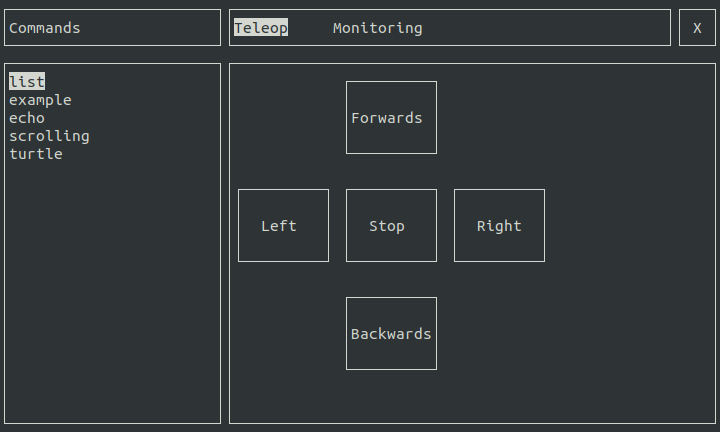
\includegraphics[scale=0.6]{Teleop}
  \caption{Screenshot of application showing the teleoperation interface}
  \label{fig:teleop}
\end{figure}

\newpage

The buttons themselves are sub-windows of the main output window. The reason for this is that it was easier to draw a box around them. Also, this makes it easier to determine if a mouse click was registered inside a button due to the {\fontfamily{pcr}\selectfont ncurses} function {\fontfamily{pcr}\selectfont wmouse}\_trafo. The function that defines the positions of each button is unfortunately long and overly complex. It also uses hard coded values for the button dimensions and the button labels. However, it effectively sizes the buttons appropriately and ensures that the label is kept in the middle of the button by forcing the vertical size to be an odd number.

In order to integrate the teleoperation tab into the tab bar, it was decided to keep it as the first index at all times. The menu printing function was modified to accept an extra vector of strings to prefix the start of the list. Additionally, it was hard coded that if the bar index was at 1, this indicated that teleoperation mode was active.

The user interface responds to teleoperation mode by displaying the teleoperation tab in the main window. Additionally, this allows the user to control the robot using the keyboard or on-screen buttons.

\subsection{Monitoring Tab}
\label{monitor_ui}

As explained in Section \ref{monitoring}, the monitoring tab was created as a static output displaying pre-defined sets of data. The UI comprises of two sections (Telemetry and Safety) containing lists of message data with preceding labels. As the interface is hard coded, the method of printing is not exactly elaborate, apart from the way that coloured boxes are displayed.

Colour-coded boxes are used for some items as opposed to raw data for a more visual representation of the robot status. This works by defining colour pairs for green, yellow and red, and assigning each to numbers. The number that is used is then based on the message value provided. As a precaution, any number outside of the expected range is treated as green by default. A box is then drawn by enabling the correct colour pair before printing two spaces which creates a square. A screenshot of the final version is shown below:

\begin{figure}[h!]
  \centering
  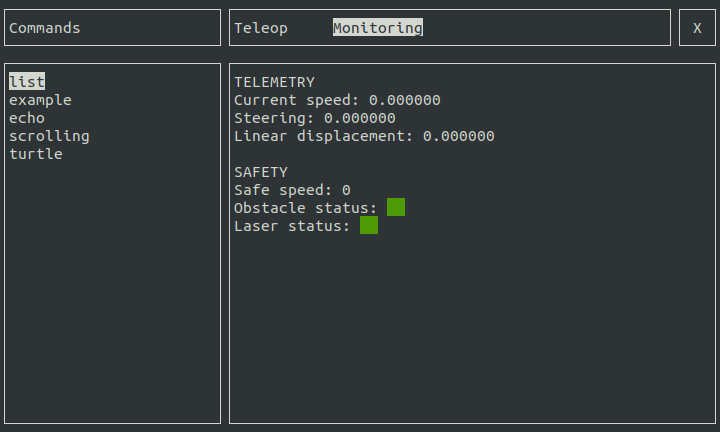
\includegraphics[scale=0.6]{Monitor}
  \caption{Screenshot of the monitoring interface}
  \label{fig:monitor}
\end{figure}

\section{Process Management}
\label{process_management}

\subsection{Starting Processes}
\label{starting_processes}

The application reads the {\fontfamily{pcr}\selectfont YAML} configuration file during its initialisation. Part of this file defines the commands to be made available in the menu and run within the program. The file is parsed using {\fontfamily{pcr}\selectfont yaml-cpp}\cite{yaml-cpp} and each process is constructed with the data extracted from there. The file was originally using a custom format until it was decided that this would be too complicated and unnecessary. Also {\fontfamily{pcr}\selectfont YAML} is used heavily in {\fontfamily{pcr}\selectfont ROS} so using it for this application seemed more suitable than alternatives for the sake of consistency. Additionally, {\fontfamily{pcr}\selectfont yaml-cpp} is the actual library used by {\fontfamily{pcr}\selectfont ROS} to interpret {\fontfamily{pcr}\selectfont YAML} files. This means that on some systems, there is no need to install it as a separate dependency (although this was not consistently true). It was also decided to separate the program executable option from the parameter option in the file. This makes parsing easier due to the increased ability to deal with commands that do not use parameters.

The location of the {\fontfamily{pcr}\selectfont YAML} file is initially presumed to be in the ".config" directory as this is standard for most Unix applications. However, if this is not present, the provided sample file is read as a temporary alternative.

In order to start a process, the strings in the {\fontfamily{pcr}\selectfont YAML} file need to be split in order to extract the executable name and the separate parameters to be passed to {\fontfamily{pcr}\selectfont execv}\cite{exec}. This was done using the {\fontfamily{pcr}\selectfont boost}\cite{boost} split algorithm, splitting by spaces or "/" characters where appropriate. This was planned to be done manually using {\fontfamily{pcr}\selectfont strtok}, however, due to complications, it was decided to make use of pre-made libraries. This made the relevant sections of code simpler and ultimately saved development time. There were also some initial problems regarding accepting zero or multiple parameters. However, these were alleviated by making use of both {\fontfamily{pcr}\selectfont yaml-cpp} and the {\fontfamily{pcr}\selectfont boost} split algorithm and is now functioning properly.

When the necessary process information has been extracted from the configuration file, the desired process is run when it is selected from the menu. This is done by forking the program and running the {\fontfamily{pcr}\selectfont execv} function. Specifically, the program uses {\fontfamily{pcr}\selectfont forkpty}\cite{forkpty} which forks as well as creates a new pseudo-terminal simultaneously. This streamlines the common practice of doing this manually with arguably verbose code. Before introducing pseudo-terminals as described in Section \ref{section:pty}, the regular {\fontfamily{pcr}\selectfont fork} function was used originally before the change in design decision.

\subsection{Emulating Teletype Interfaces}
\label{section:pty}

An unforeseen issue surfaced while testing the application using {\fontfamily{pcr}\selectfont ROS} commands such as {\fontfamily{pcr}\selectfont roscore} and {\fontfamily{pcr}\selectfont roslaunch}. This issue was primarily to do with how {\fontfamily{pcr}\selectfont ROS} utilities (as well as other programs) display and manipulate data in the terminal. In order to display text in colour without explicitly using ASCII escape codes, as well as accept standard input as raw input, these programs change the {\fontfamily{pcr}\selectfont termios} attributes of their respective terminal devices. If a program does this to suit its own needs, the parent application does not accept user input as the {\fontfamily{pcr}\selectfont ncurses} settings were being overridden by the children.

The solution to this problem was to essentially emulate a Teletype interface {\fontfamily{pcr}\selectfont (TTY)} using pseudo-terminals {\fontfamily{pcr}\selectfont (PTY's)}\cite{pty} for each child process so that they act as if they are running in a regular terminal environment. Additionally, it was necessary to disable standard input for each {\fontfamily{pcr}\selectfont PTY} so that the parent can take over. Much of the understanding and the actual code for this came from a project called {\fontfamily{pcr}\selectfont tty8}\cite{tty8}, an example of which can be found in Appendix \ref{appendix:c}.

The example shown illustrates how standard input as well as blocking were disabled as the process was being started. As well as this, during the creation of the {\fontfamily{pcr}\selectfont PTY}, the original signal mask was passed as a parameter in order to preserve the terminal attributes of the parent. This resulted in a positive outcome in which {\fontfamily{pcr}\selectfont ROS} processes were not interrupting the activity of the parent, allowing for effective multitasking and the ability to use the application as intended.

A subsequent benefit of this problem being solved was that the colour data that {\fontfamily{pcr}\selectfont ROS} outputs was being captured in its raw form where previously it was being omitted from the text. This creates the opportunity to parse and convert text into its intended colour in the main output screen using {\fontfamily{pcr}\selectfont ncurses} colour pairs during the printing stage. Unfortunately, due to time constraints this was not implemented and instead the codes are deleted using a regular expression. This makes use of the {\fontfamily{pcr}\selectfont regex}\cite{cpp-regex} standard library and does remove most of the undesired meta-data. There are some matches that are not consistent with other testing that was performed using a {\fontfamily{pcr}\selectfont regex} tester\cite{regex-tester} for unknown reasons. As a result there are some visible escape codes that are not too noticeable but are not removable for some unknown reason.

Another improvement that using pseudo-terminals made was the resolution of an issue identified during earlier development. The issue occurred when there were multiple tabs open and the user closes a tab that is to the left of any other tab. This resulted in the output of the tab that was to the right of the closed tab to stall indefinitely. The issue was non-existent after introducing pseudo-terminals even though the direct cause was never determined.

One problem with the way pseudo-terminals were being created was discovered later in development and was found to be the cause of major issues. Essentially, the original terminal settings that were passed to {\fontfamily{pcr}\selectfont forkpty} was being stored before the {\fontfamily{pcr}\selectfont ncurses} environment was initialised. This means that it was not using the terminal attributes set by {\fontfamily{pcr}\selectfont ncurses} but rather the settings used before initialisation. This, combined with not properly setting signal settings on the side of the parent, lead to undefined behaviour and complete crashing. This usually occurred when trying to use the mouse as described in Section \ref{sidebar_menu} and made any hope of using the mouse potentially dangerous. The issue was also leading to inconsistent output behaviour such as randomly making all output upper-case. The issue has since been properly resolved and the mouse input behaves as expected.

\subsection{Capturing Process Output}
\label{capturing_output}

An initial design decision was to use {\fontfamily{pcr}\selectfont popen}\cite{popen} in order to combine forking and running {\fontfamily{pcr}\selectfont exec} and {\fontfamily{pcr}\selectfont fdopen}\cite{fdopen} into one function. However, due to a misunderstanding as to how {\fontfamily{pcr}\selectfont popen} works, it was found to be unhelpful for certain features of the application. The reason for this is that {\fontfamily{pcr}\selectfont popen} does not return the process ID of the forked process which means that it is impossible to reliably kill it. The only way to use this would be to kill processes with {\fontfamily{pcr}\selectfont pkill}\cite{pkill} which kills all processes matching a regular expression which is not ideal. This meant that it was necessary to re-implement the functionality of {\fontfamily{pcr}\selectfont popen} in order to gain access to both the standard output and the {\fontfamily{pcr}\selectfont PID} of each process. This served to delay development as well as make the code more complicated than initially predicted. However, this re-implementation meant that solving a later issue \ref{section:pty} was easier due to more granular control over the functionality.

In order to display process output properly, it needs to be redirected, captured and stored appropriately. This was done using {\fontfamily{pcr}\selectfont fdopen} to create a file stream that captures the file descriptor of a pseudo-terminal. This is done for each respective process that is run. In order to get the data from the file stream, {\fontfamily{pcr}\selectfont fgets} was used as it terminates either at a newline character or after a specified amount of characters. This is helpful because if the size of the window is given to it, this results in line wrapping built in to the function. This is performed for every process in the tab bar iteratively. An example of line wrapping is shown in the screenshot below:

\begin{figure}[h!]
  \centering
  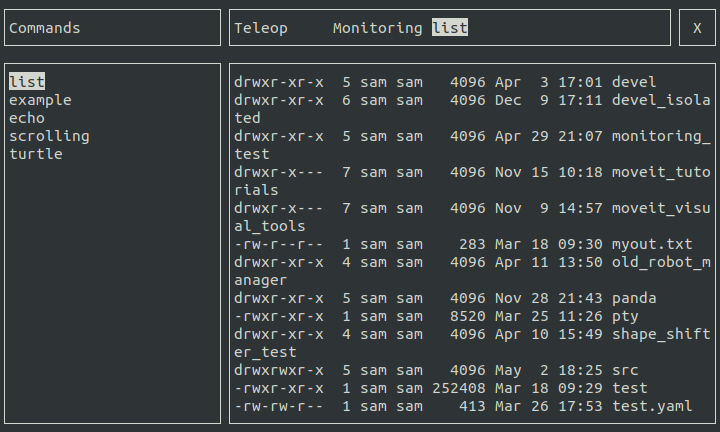
\includegraphics[scale=0.6]{TrueOutput}
  \caption{Screenshot of the {\fontfamily{pcr}\selectfont ls} program output being displayed and wrapped}
  \label{fig:output}
\end{figure}

Before the implementation of pseudo-terminals as described in Section \ref{section:pty}, the output redirection was being done with pipes and the {\fontfamily{pcr}\selectfont dup2} function. There were some initial issues with redirecting the file descriptors correctly as it is not well explained in the documentation. Also, before the discovery of the {\fontfamily{pcr}\selectfont fdopen} utility, there was an attempt to recreate {\fontfamily{pcr}\selectfont fgets} using the read function. This turned out to be a waste of time and was not successful regardless of the inclusion of {\fontfamily{pcr}\selectfont fdopen}.

\subsection{Killing Processes}
\label{killing}

An integral and simultaneously temperamental aspect of this project is to be able to kill processes easily. The way this was being done initially was to send a kill signal using {\fontfamily{pcr}\selectfont SIGINT} and then wait for the given process to terminate. The advantage of this is that the program can take note of the death of a process and prevent it from remaining in a zombie state. However, a particular problem with {\fontfamily{pcr}\selectfont ROS} applications is that they need to shut down safely and thus take a long time to terminate. The result of this is that the parent application that is waiting for them to terminate is completely frozen. However, since learning about options that can be passed to {\fontfamily{pcr}\selectfont waitpid}, a subroutine was added to keep track of terminated processes and subsequently wait for each of them and remove them once each process has fully terminated. This made killing {\fontfamily{pcr}\selectfont ROS} processes safer, more reliable and less likely to halt the parent application.

\section{Teleoperation}
\label{teleop}

This section describes the back-end implementation of the teleoperation feature. The general function of this is to construct and send geometry twist messages to a given {\fontfamily{pcr}\selectfont ROS} topic. The message that is sent will be adjusted based on user input, changing the linear velocity and the turning increment. Each button press will add an amount to the relevant velocities in question.

In order to ensure that the robot can be straightened, it was made so the turning value will degrade to zero over time. This allows the robot to continue to drive in a straight line if no alterations are made. This occurs iteratively after a given amount of time and subtracts a given amount from the velocity before sending a message. Without this delay, it was found that turning is impossible due to the main loop being too fast.

If the stop function is called, a linear and rotational velocity of 0 will be published ten times. This was a suggested amount given by the project supervisor based on the behaviour of the systems already in place. Sending multiple stop messages simply ensures that at least one will be received by the robot and is a point of precaution.

One issue discovered during hardware testing was that velocity messages were being sent out far too quickly, leading to lag and a large message queue. This was due to the fact that messages were being re-sent during each iteration of the main loop without any sort of delay. Messages have to be sent constantly during teleoperation in order to maintain control, however the lack of delay was causing problems for other applications. The solution to this was to add a timer to the refresh function that will tick over after a configured amount of seconds. The value of the amount of time to wait is defined in the configuration file which gives the user the ability to adjust it according to the needs of the hardware being used. Additionally, it was found that the queue for the {\fontfamily{pcr}\selectfont ROS} publisher was too large at 100 and should have been set to 10 to further limit the amount of messages that are sent at any one time.

An emergent behaviour of having two message sending timers is that, of course only one of them is going to be useful. That would be the time that is the smallest which does make the second timer redundant. That being said, the functionality of each is technically different given that one timer reduces rotational velocity as well as sends messages. So, depending on the system, it may be worth setting one higher than the other, meaning that the option is there if needed.

Much of the teleoperation behaviour is dependent on the configuration file as it defines the following attributes:

\begin{itemize}
  \item The amount of time to wait between sending regular messages
  \item The topic to publish to
  \item The magnitude of the rotational degradation
  \item The amount of time to wait between degrading the rotation
  \item The magnitude of the linear and rotational velocities to be added on for every button press
\end{itemize}

An example set of values can be viewed in the teleop section of the example configuration file in Appendix \ref{appendix:c}.

A feature that was also implemented was a teleoperation mode that would disable when not on the teleoperation tab of the interface. Disabling this mode means that no messages will be sent which allows other {\fontfamily{pcr}\selectfont ROS} processes to take control of the robot without interruption. There was an issue with this function where, while switching tabs will send a stop signal, the previous velocity before the switch was somehow being stored. This lead to the robot resuming movement when switching back to the teleoperation tab. This issue was solved by sending more stop signals and being more strict when entering and leaving teleoperation mode.

An unfortunate consequence of having one application that can control robots as well as manage processes is that it still has to be a {\fontfamily{pcr}\selectfont ROS} node. As such, it requires {\fontfamily{pcr}\selectfont roscore} to be running before it is started which is unfortunate as it means that the output of {\fontfamily{pcr}\selectfont roscore} cannot be monitored in a tab. This issue was discovered late in development and is unfortunately not fixable given the nature of {\fontfamily{pcr}\selectfont ROS}. A suggested solution was to use {\fontfamily{pcr}\selectfont roslaunch} to launch the application as it automatically runs {\fontfamily{pcr}\selectfont roscore}. Unfortunately, due to the way that {\fontfamily{pcr}\selectfont roslaunch} changes the terminal settings, the application simply froze and did not work at all.

\section{Monitoring}
\label{monitoring}

The monitoring interface was initially designed to be a variable number of tabs that could be configured extensively to display any {\fontfamily{pcr}\selectfont ROS} topic data. However, due to a combination of factors, the interface was implemented as a static layout that displays pre-defined message types. One reason for this was time constraints nearing the end of development as well as complications involving subscribing to generic message types. Syntactically, {\fontfamily{pcr}\selectfont ROS} has no way to do this in {\fontfamily{pcr}\selectfont C++} as the callback message parameter needs to have a declaration of its message type.

There was an attempt at using shapeshifters\cite{shapeshifter}, however, the dependencies for doing this were not functional. While accomplishing something similar to this is possible, it was decided to create a monitoring tab that was suitable enough for Idris. The topics to subscribe to are defined in the configuration file and messages are checked for iteratively in the main loop. The back end of this process not exactly complex, although there are some interesting front end concepts described in Section \ref{monitor_ui}.
